 \documentclass[rgb]{beamer}
\usepackage{silence,lmodern}
\usepackage[backend=biber, style=ieee]{biblatex}
\usepackage{csquotes}
\usepackage{listings}
\usepackage{svg}
\usepackage{multirow}
\usepackage{multicol}

\WarningFilter{biblatex}{Patching footnotes failed}
\WarningFilter{etex}{Extended allocation already in use}

\renewcommand*{\bibfont}{\tiny}
\bibliography{ressources.bib}

\usetheme{Konstanz}
\setcounter{secnumdepth}{3}
\format{169}

\makeatletter
\def\thickhline{%
  \noalign{\ifnum0=`}\fi\hrule \@height \thickarrayrulewidth \futurelet
  \reserved@a\@xthickhline}
\def\@xthickhline{\ifx\reserved@a\thickhline
              \vskip\doublerulesep
              \vskip-\thickarrayrulewidth
            \fi
     \ifnum0=`{\fi}}
\makeatother
 
\newlength{\thickarrayrulewidth}
\setlength{\thickarrayrulewidth}{4\arrayrulewidth}


\title{Label Hierarchy Inference in Property Graph Databases}
\titleCorporateDesign{Label Hierarchy}{Inference in}{Property Graph}{Databases}
\author{Fabian Klopfer} 
\date{\today}
\institute{Databases and Information Systems Chair \\ University of Konstanz}

\begin{document}

\setmainfont{Arial}
\setsansfont{Arial}
\usebeamerfont{normalfont}



\begin{frame}
	\titlepage
\end{frame}

\section{Introduction}

        \begin{frame}[t]{Running Example}
        Simple example, with no overlapping labels and a perfect hierarchy: \\
        
        \vspace{1cm}
        
        \centering\begin{tabular}{|c|c|} \hline
             Node.name & Node.labels \\ \thickhline
            Fernando's & restaurant, italian \\ \hline
            Arche & restaurant, vietnamese \\ \hline
            Bangkok & restaurant, thai \\ \hline
            CampusCafe & cafe, wifi \\ \hline
            Endlicht & cafe, latenight \\ \hline
            Pano & cafe, breakfast \\ \hline
            Lago & shopping, mall \\ \hline
            Seerhein Center & shopping, cheap \\ \hline
            Seepark & Shopping, expensive \\ \hline
        \end{tabular}
        \end{frame}{}

    \subsection{Motivation}
        \begin{frame}[allowframebreaks]
        \subsectionpage
        \begin{itemize}
            \item Implicit hierarchical structure in many data sets
            \item implicit in property graph
            \item no explicit representation in Neo4J or the property graph model
        \end{itemize}        
        \vspace{0.8cm}
        In practice it may help:
        \vspace{0.8cm}
            \begin{itemize}
                \item Missing labels \& other data impurities can be fixed
                \item Neo4J cardinality estimation can be improved
                \item and many others
            \end{itemize}{}
            \vspace{0.8cm}
            However that's not what is dealt with here
        \end{frame}
        


    \subsection{Problem Definition}
        \begin{frame}[fragile]
            \subsectionpage
            \begin{multicols}{2}
            Given: Set of labels $\{ l_i, l_j, l_k, \dots \}$ \\
            Wanted: Taxonomy/Hierarchy of labels  \\
            \vspace{0.8cm}
            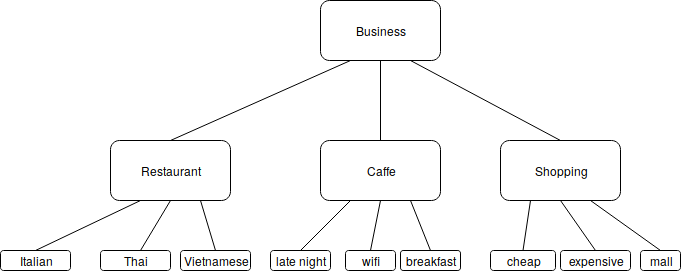
\includegraphics[keepaspectratio,width=\columnwidth]{graphics/aproaches/ex_hierarchy.png} \\
            \vfill\null
            \columnbreak
            
            \begin{tabular}{|c|c|} \hline
                 Node.name & Node.labels \\ \thickhline
                Fernando's & restaurant, italian \\ \hline
                Arche & restaurant, vietnamese \\ \hline
                Bangkok & restaurant, thai \\ \hline
                CampusCafe & cafe, wifi \\ \hline
                Endlicht & cafe, latenight \\ \hline
                Pano & cafe, breakfast \\ \hline
                Lago & shopping, mall \\ \hline
                Seerhein Center & shopping, cheap \\ \hline
                Seepark & Shopping, expensive \\ \hline
            \end{tabular}
            \end{multicols}
           
            
        \end{frame}
        


\section{Solutions: Hierarchical Clustering}
    \subsection{Approaches}
    \begin{frame}
        \sectionpage
        \subsectionpage
        \vspace{1cm}
        3 different approaches were considered:
        \vspace{0.48cm}
        \begin{enumerate}
            \item Agglomerative clustering
            \item Two-step clustering
            \item Conceptual clustering
        \end{enumerate}
        \vspace{0.48cm}
       
        \end{frame}
        
    \begin{frame}{Common for 1  \& 2}
        \begin{itemize}
            \item Each data instance is set of labels
            \item distance measure is set similarity e.g. jaccard or l1 on vectorized representation
            \item Dendrograms got flattened
        \end{itemize}
        
        \centering\begin{tabular}{|c|c|} \hline
             Node.name & Node.labels \\ \thickhline
            Fernando's & restaurant, italian \\ \hline
            Arche & restaurant, vietnamese \\ \hline
            Bangkok & restaurant, thai \\ \hline
            CampusCafe & cafe, wifi \\ \hline
            Endlicht & cafe, latenight \\ \hline
            Pano & cafe, breakfast \\ \hline
            Lago & shopping, mall \\ \hline
            Seerhein Center & shopping, cheap \\ \hline
            Seepark & Shopping, expensive \\ \hline
        \end{tabular}
    \end{frame}
        
    \begin{frame}{Single Linkage Clustering}
        Merge the two clusters with the smallest distance per cluster/set of labels \\
        Implementation of SciPy \cite{scipy} \\
        In the following: Enhanced plots and result trees: \alert{non-standard single linkage!} \\
        \centering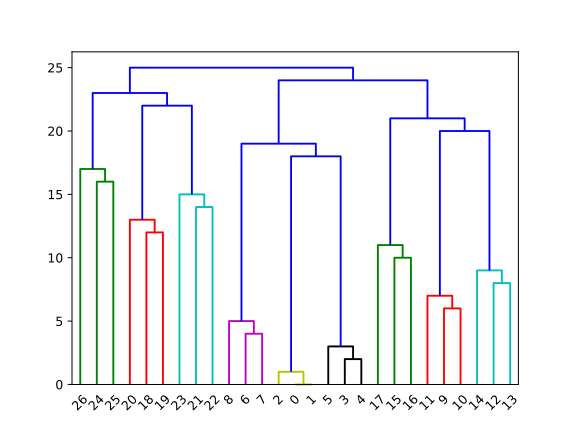
\includegraphics[keepaspectratio,width=\textwidth, height=0.7\textheight]{graphics/aproaches/single_noise_False_equi_dendro.png} \hspace{2cm}
        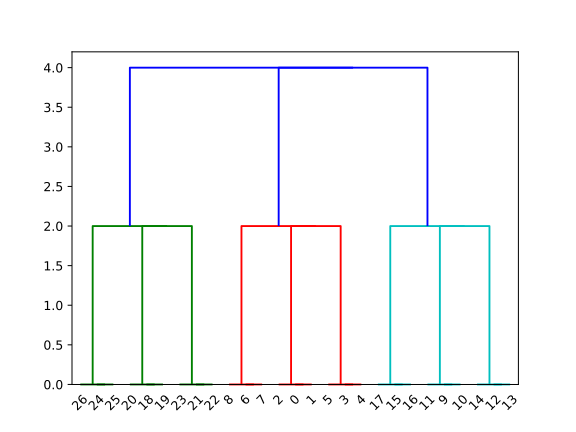
\includegraphics[keepaspectratio,width=\textwidth, height=0.7\textheight]{graphics/aproaches/single_noise_False_dendro.png}
        \end{frame}
        
    \begin{frame}{Two-step clustering}
        Idea: reduce number of observations by other clustering and then do hierarchical clustering. \\
        Implementations as before, plus Scikit-Learn \cite{scikit-learn} and PyClustering \cite{Novikov2019}. \\
        \centering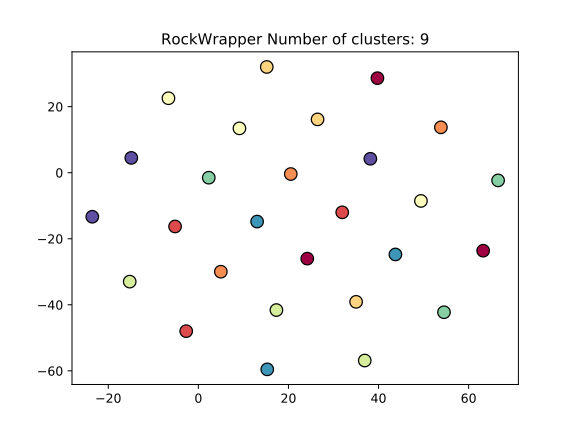
\includegraphics[keepaspectratio,width=\textwidth, height=0.7\textheight]{graphics/aproaches/rock_noise_False_clusters.png}  \hspace{2cm}
        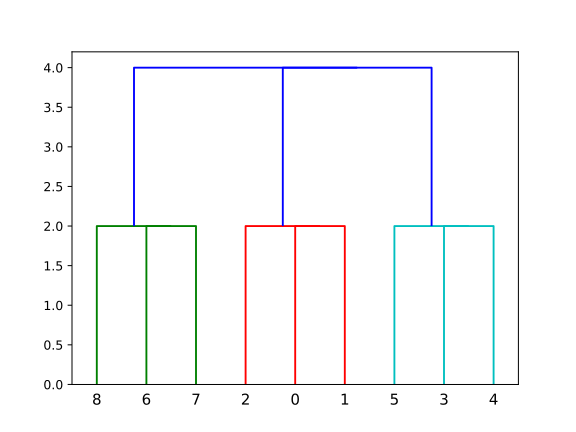
\includegraphics[keepaspectratio,width=\textwidth, height=0.7\textheight]{graphics/aproaches/rock_noise_False_dendro.png}
    \end{frame}
    
        \begin{frame}{Conceptual clustering}
        Idea: Build a hierarchy of label sets/concepts with descriptions and integrate instances iteratively, splitting when too distinct \\
        Comparable to decision trees, form of divisive clustering. 
        Implementation of MacLellan et al. \cite{trestle:2016a} \\
        \centering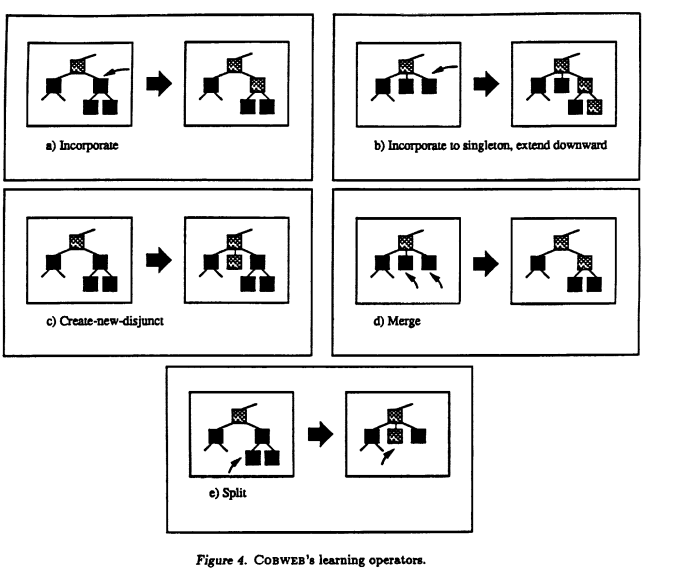
\includegraphics[keepaspectratio,width=0.48\textwidth,height=0.6\textheight]{graphics/aproaches/cobweb_ops.png} \hspace{2cm}
        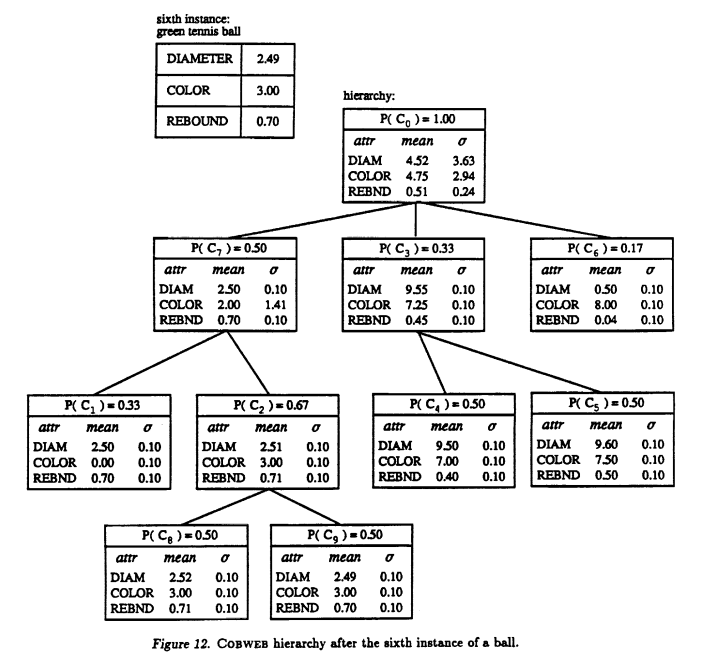
\includegraphics[keepaspectratio,width=0.48\textwidth,height=0.6\textheight]{graphics/aproaches/cobweb_ex.png}
    \end{frame}

\section{Evaluation}
    \subsection{Setup}
        \begin{frame}[fragile]
        \subsectionpage
         noise $\equiv$ take a node and remove $\vee$ rename a label \\

        \begin{lstlisting}
        "id":24,"labels":"l2, l22",
        "id":25,"labels":"l22",
        "id":26,"labels":"l1"
        \end{lstlisting}
         Run the algorithm on each of the variations:
            \begin{enumerate}
                \item no noise
                \item  $10\%$ noise
                \item $33\%$ noise
                \item $50\%$ noise
            \end{enumerate} 
            Convert the output into a bracket tree

                Metric for how much resulting hierarchy deviates from perfect: Tree Edit Distance \cite{pawlik2011rted} \cite{pawlik2016tree}
        \end{frame}
        
    \subsection{Results}
        \begin{frame}[allowframebreaks]
        \subsectionpage
            \centering 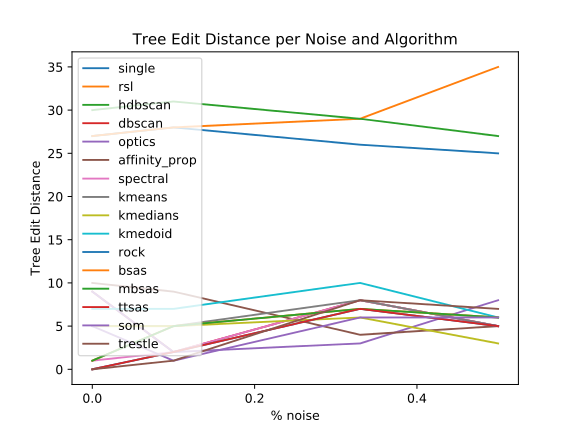
\includegraphics[keepaspectratio,width=0.48\textwidth, height=\textheight]{graphics/aproaches/ted_results.png} \hspace{0.3cm}
            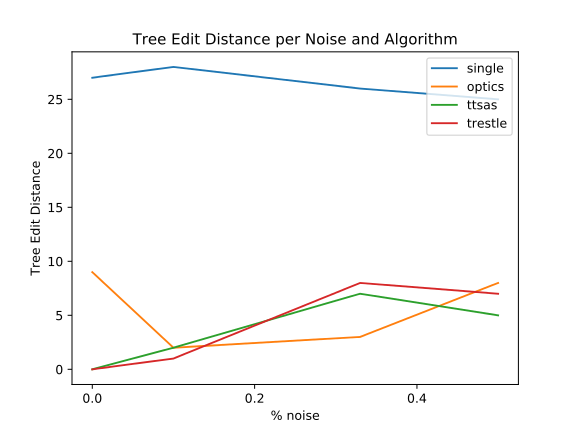
\includegraphics[keepaspectratio,width=0.48\textwidth, height=\textheight]{graphics/aproaches/ted_results_reduced.png} \\
            \framebreak
             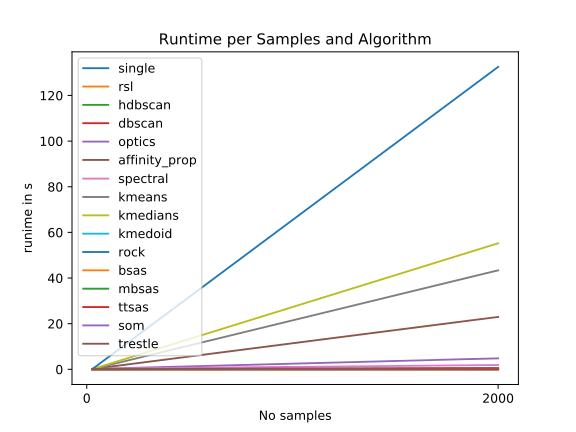
\includegraphics[keepaspectratio,width=0.48\textwidth, height=\textheight]{graphics/aproaches/time_bench.png} \hspace{0.3cm}
             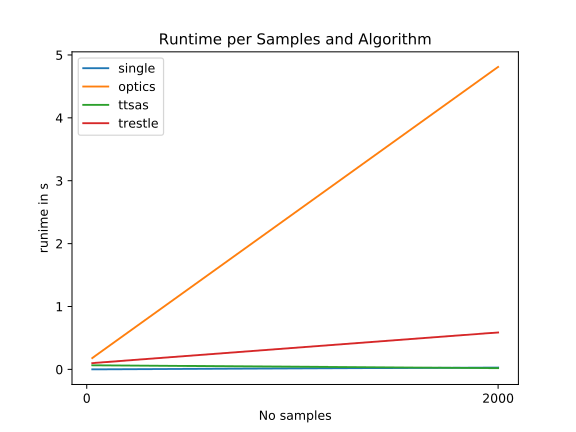
\includegraphics[keepaspectratio,width=0.48\textwidth, height=\textheight]{graphics/aproaches/time_bench_reduced.png} \\
        \end{frame}{}

        
        \begin{frame}{Agglomerative Clustering: Single Linkage}
             \centering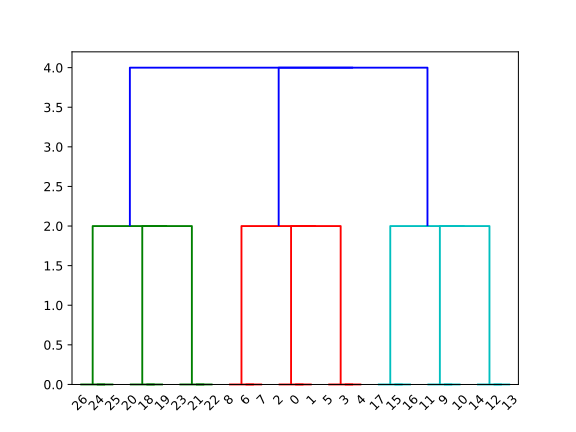
\includegraphics[keepaspectratio,width=0.48\textwidth, height=0.48\textheight]{graphics/results_single/noise_False_dendro.png} \hspace{2cm}
             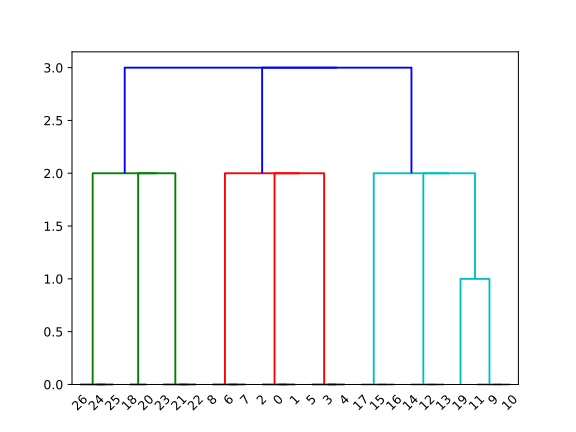
\includegraphics[keepaspectratio,width=0.48\textwidth, height=0.48\textheight]{graphics/results_single/noise_10_dendro.png} \\
            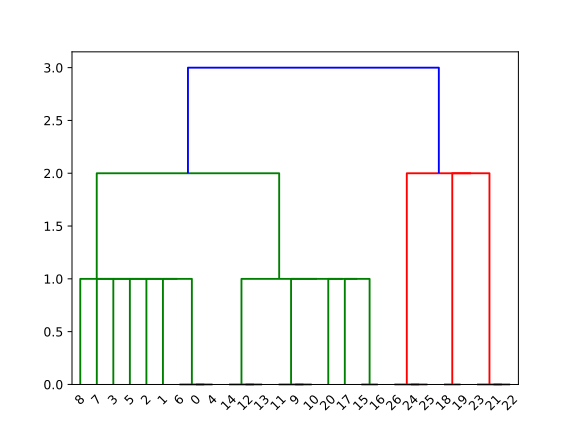
\includegraphics[keepaspectratio,width=0.48\textwidth, height=0.48\textheight]{graphics/results_single/noise_33_dendro.png} \hspace{2cm}
           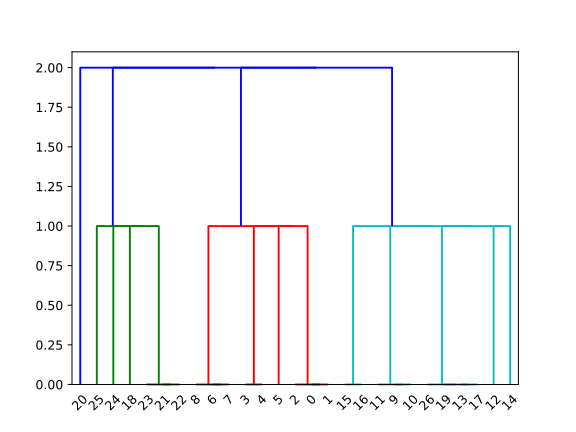
\includegraphics[keepaspectratio,width=0.48\textwidth, height=0.48\textheight]{graphics/results_single/noise_50_dendro.png}
        \end{frame}{}
        
        \begin{frame}{Two-Step Clustering: OPTICS}
           \centering  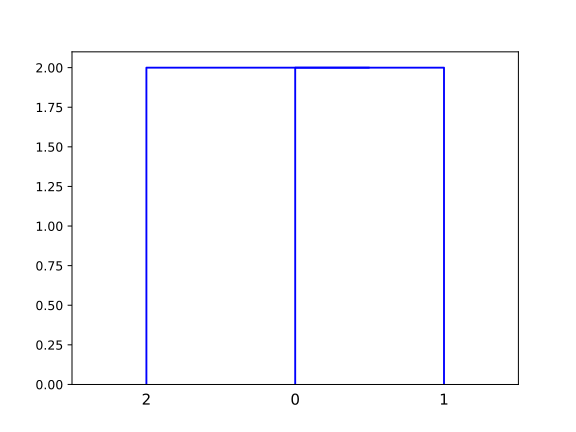
\includegraphics[keepaspectratio,width=0.48\textwidth, height=0.48\textheight]{graphics/results_two_step/noise_0_optics_dendro.png} \hspace{2cm}
             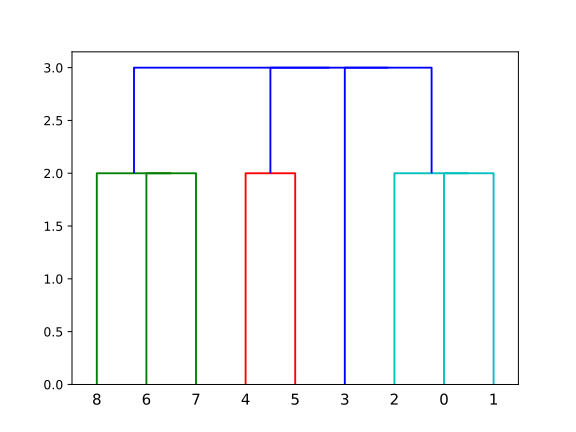
\includegraphics[keepaspectratio,width=0.48\textwidth, height=0.48\textheight]{graphics/results_two_step/noise_10_optics_dendro.png} \\
             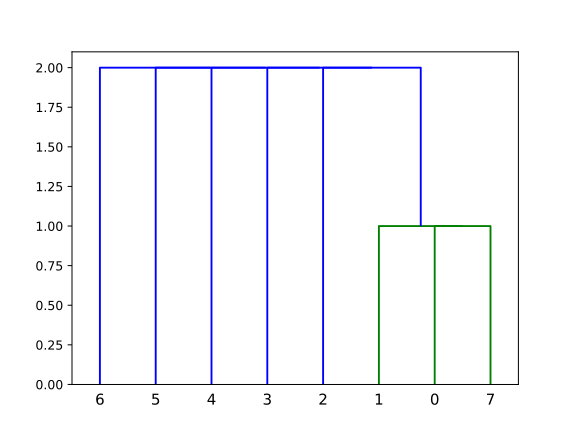
\includegraphics[keepaspectratio,width=0.48\textwidth, height=0.48\textheight]{graphics/results_two_step/noise_33_optics_dendro.png} \hspace{2cm}
             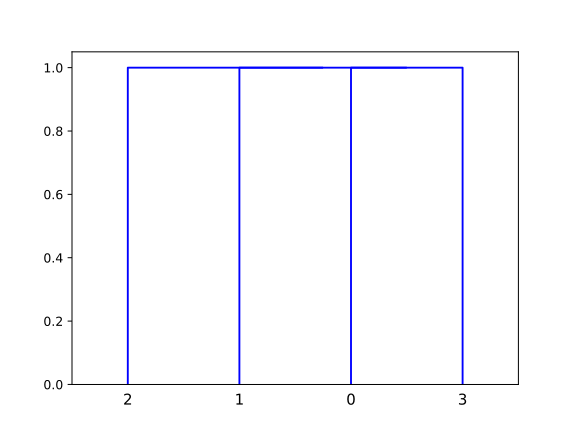
\includegraphics[keepaspectratio,width=0.48\textwidth, height=0.48\textheight]{graphics/results_two_step/noise_50_optics_dendro.png}
        \end{frame}{}

        \begin{frame}{Two-Step Clustering: TTSAS}
           \centering  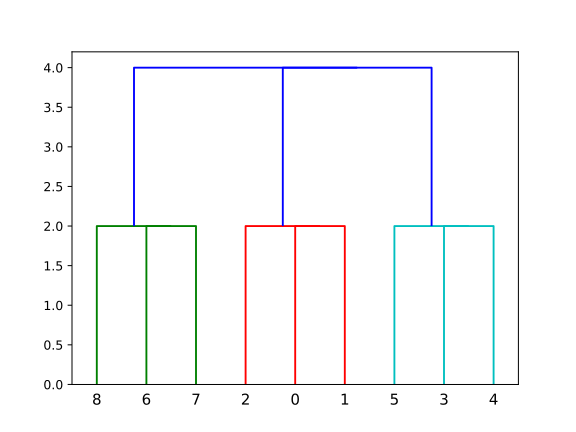
\includegraphics[keepaspectratio,width=0.48\textwidth, height=0.48\textheight]{graphics/results_two_step/noise_0_ttsas_dendro.png} \hspace{2cm}
             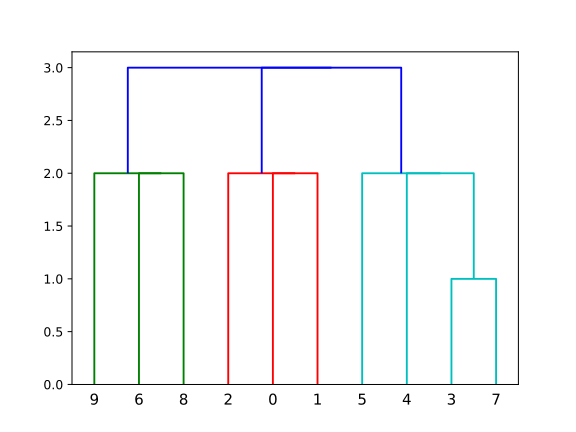
\includegraphics[keepaspectratio,width=0.48\textwidth, height=0.48\textheight]{graphics/results_two_step/noise_10_ttsas_dendro.png} \\
             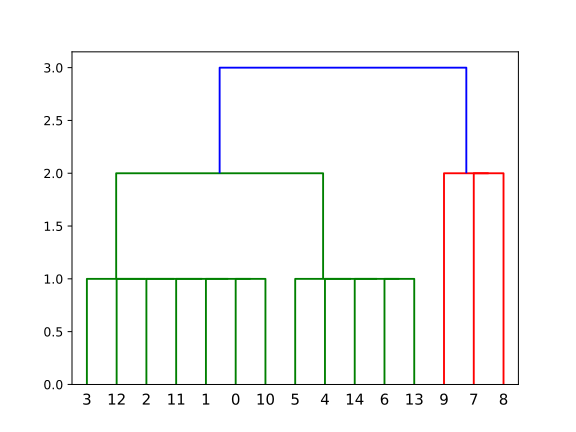
\includegraphics[keepaspectratio,width=0.48\textwidth, height=0.48\textheight]{graphics/results_two_step/noise_33_ttsas_dendro.png} \hspace{2cm}
             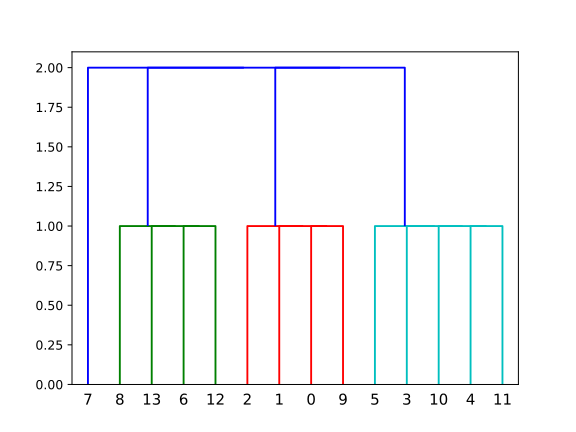
\includegraphics[keepaspectratio,width=0.48\textwidth, height=0.48\textheight]{graphics/results_two_step/noise_50_ttsas_dendro.png}
        \end{frame}{}
        
        \begin{frame}{Two-Step Clustering: SOM}
          \centering   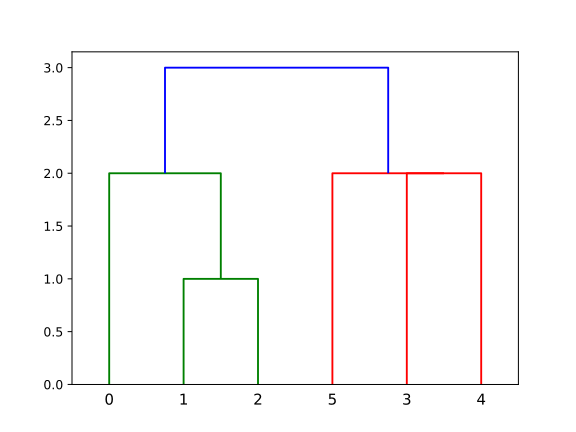
\includegraphics[keepaspectratio,width=0.48\textwidth, height=0.48\textheight]{graphics/results_two_step/noise_0_som_dendro.png} \hspace{2cm}
             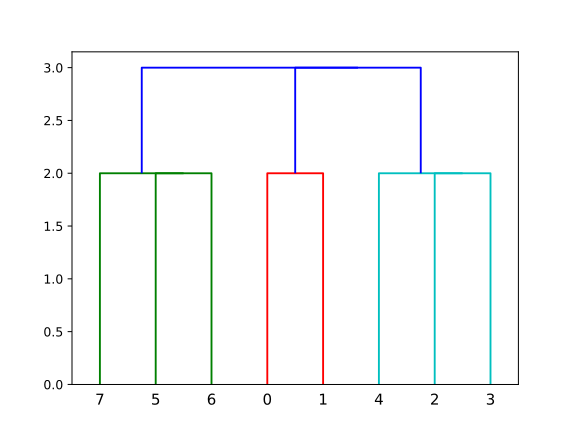
\includegraphics[keepaspectratio,width=0.48\textwidth, height=0.48\textheight]{graphics/results_two_step/noise_10_som_dendro.png} \\
             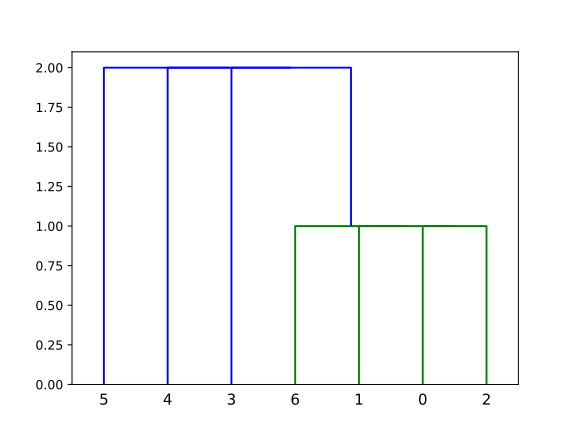
\includegraphics[keepaspectratio,width=0.48\textwidth, height=0.48\textheight]{graphics/results_two_step/noise_33_som_dendro.png} \hspace{2cm}
             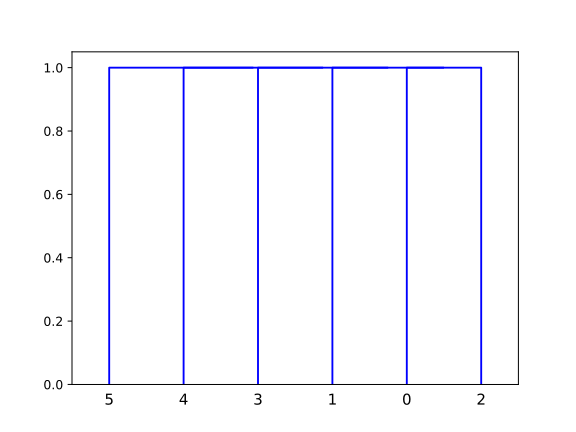
\includegraphics[keepaspectratio,width=0.48\textwidth, height=0.48\textheight]{graphics/results_two_step/noise_50_som_dendro.png}
        \end{frame}{}
        
        \begin{frame}{Conceptual Clustering: Trestle}
           \centering  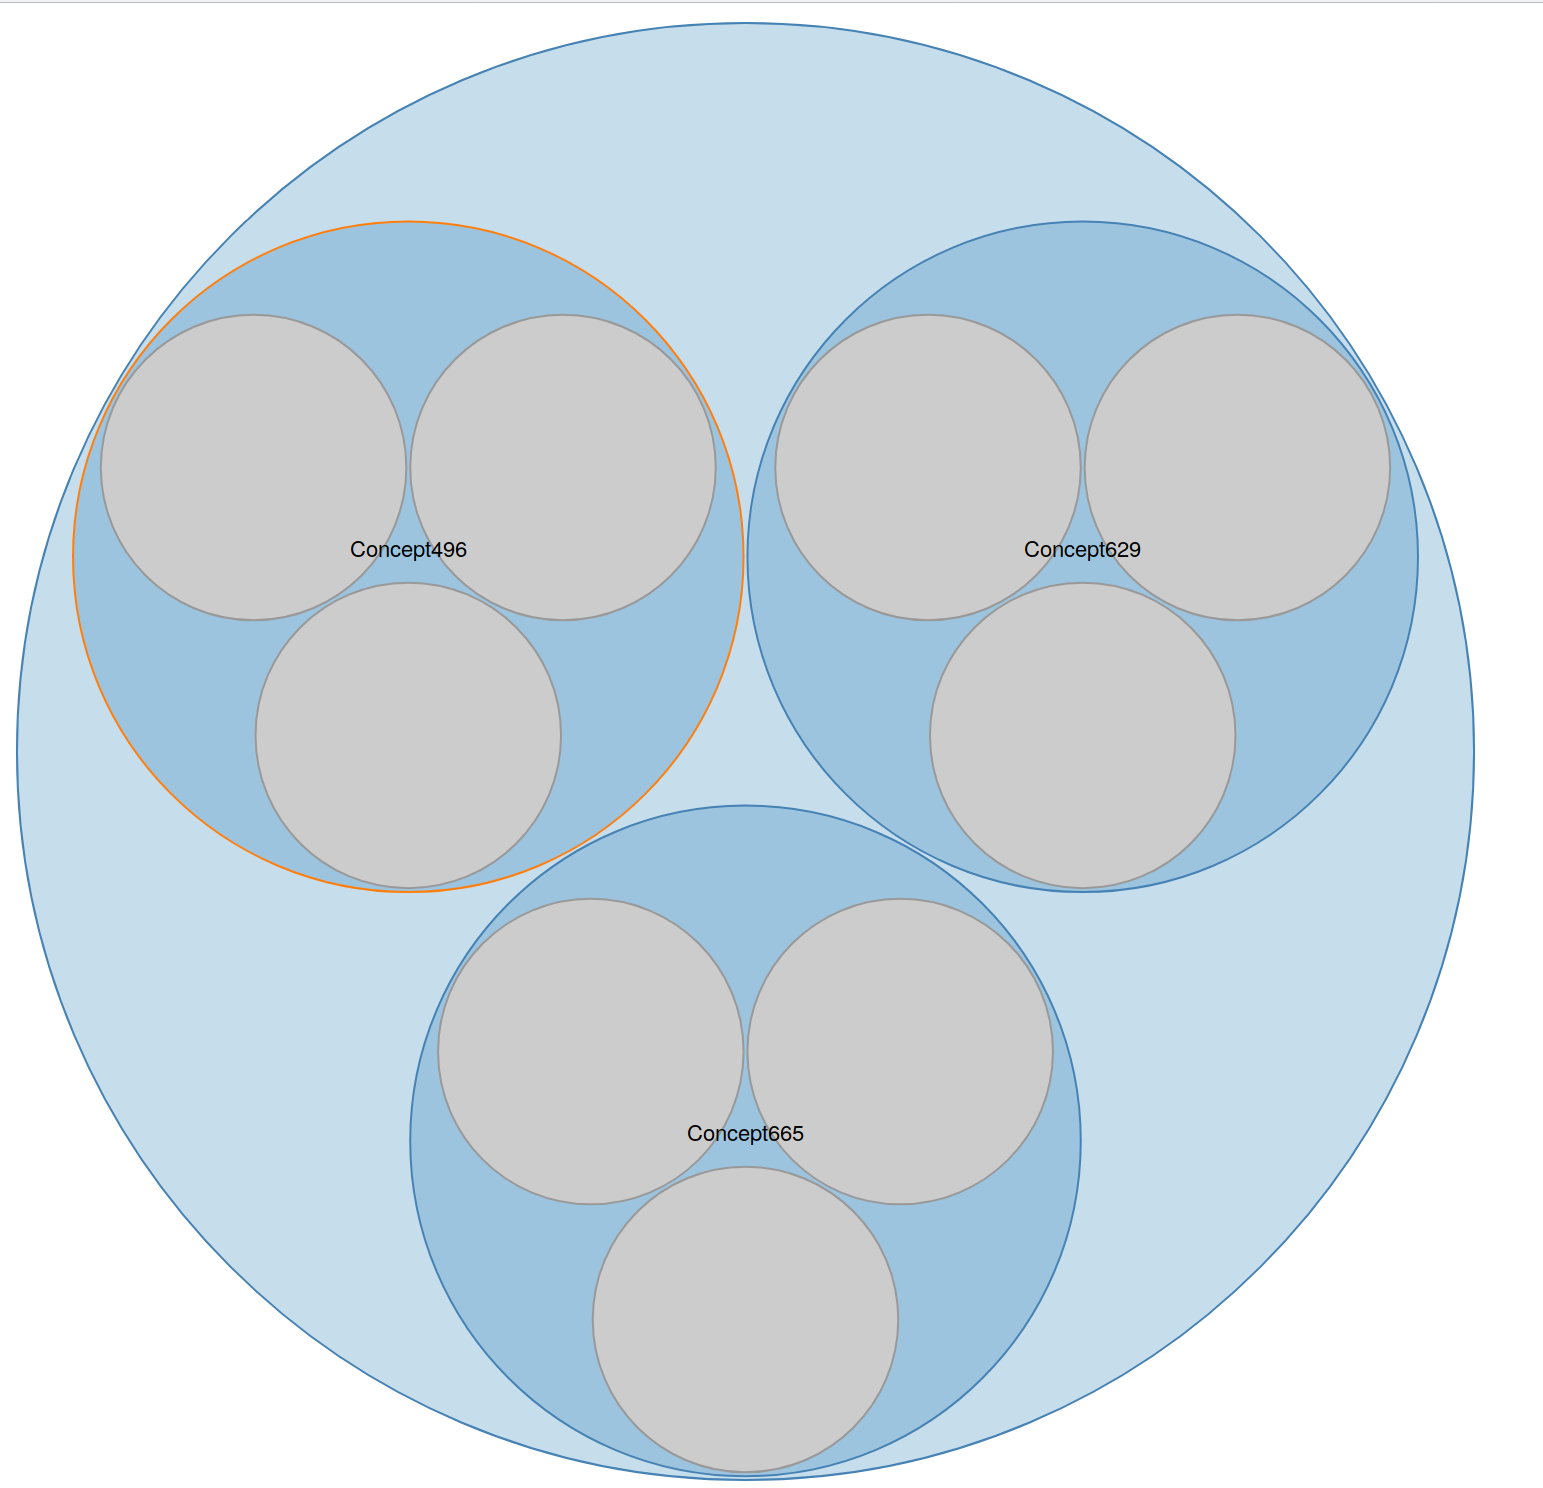
\includegraphics[keepaspectratio,width=0.48\textwidth, height=0.48\textheight]{graphics/results_trestle/trestle_0.png} \hspace{2cm}
             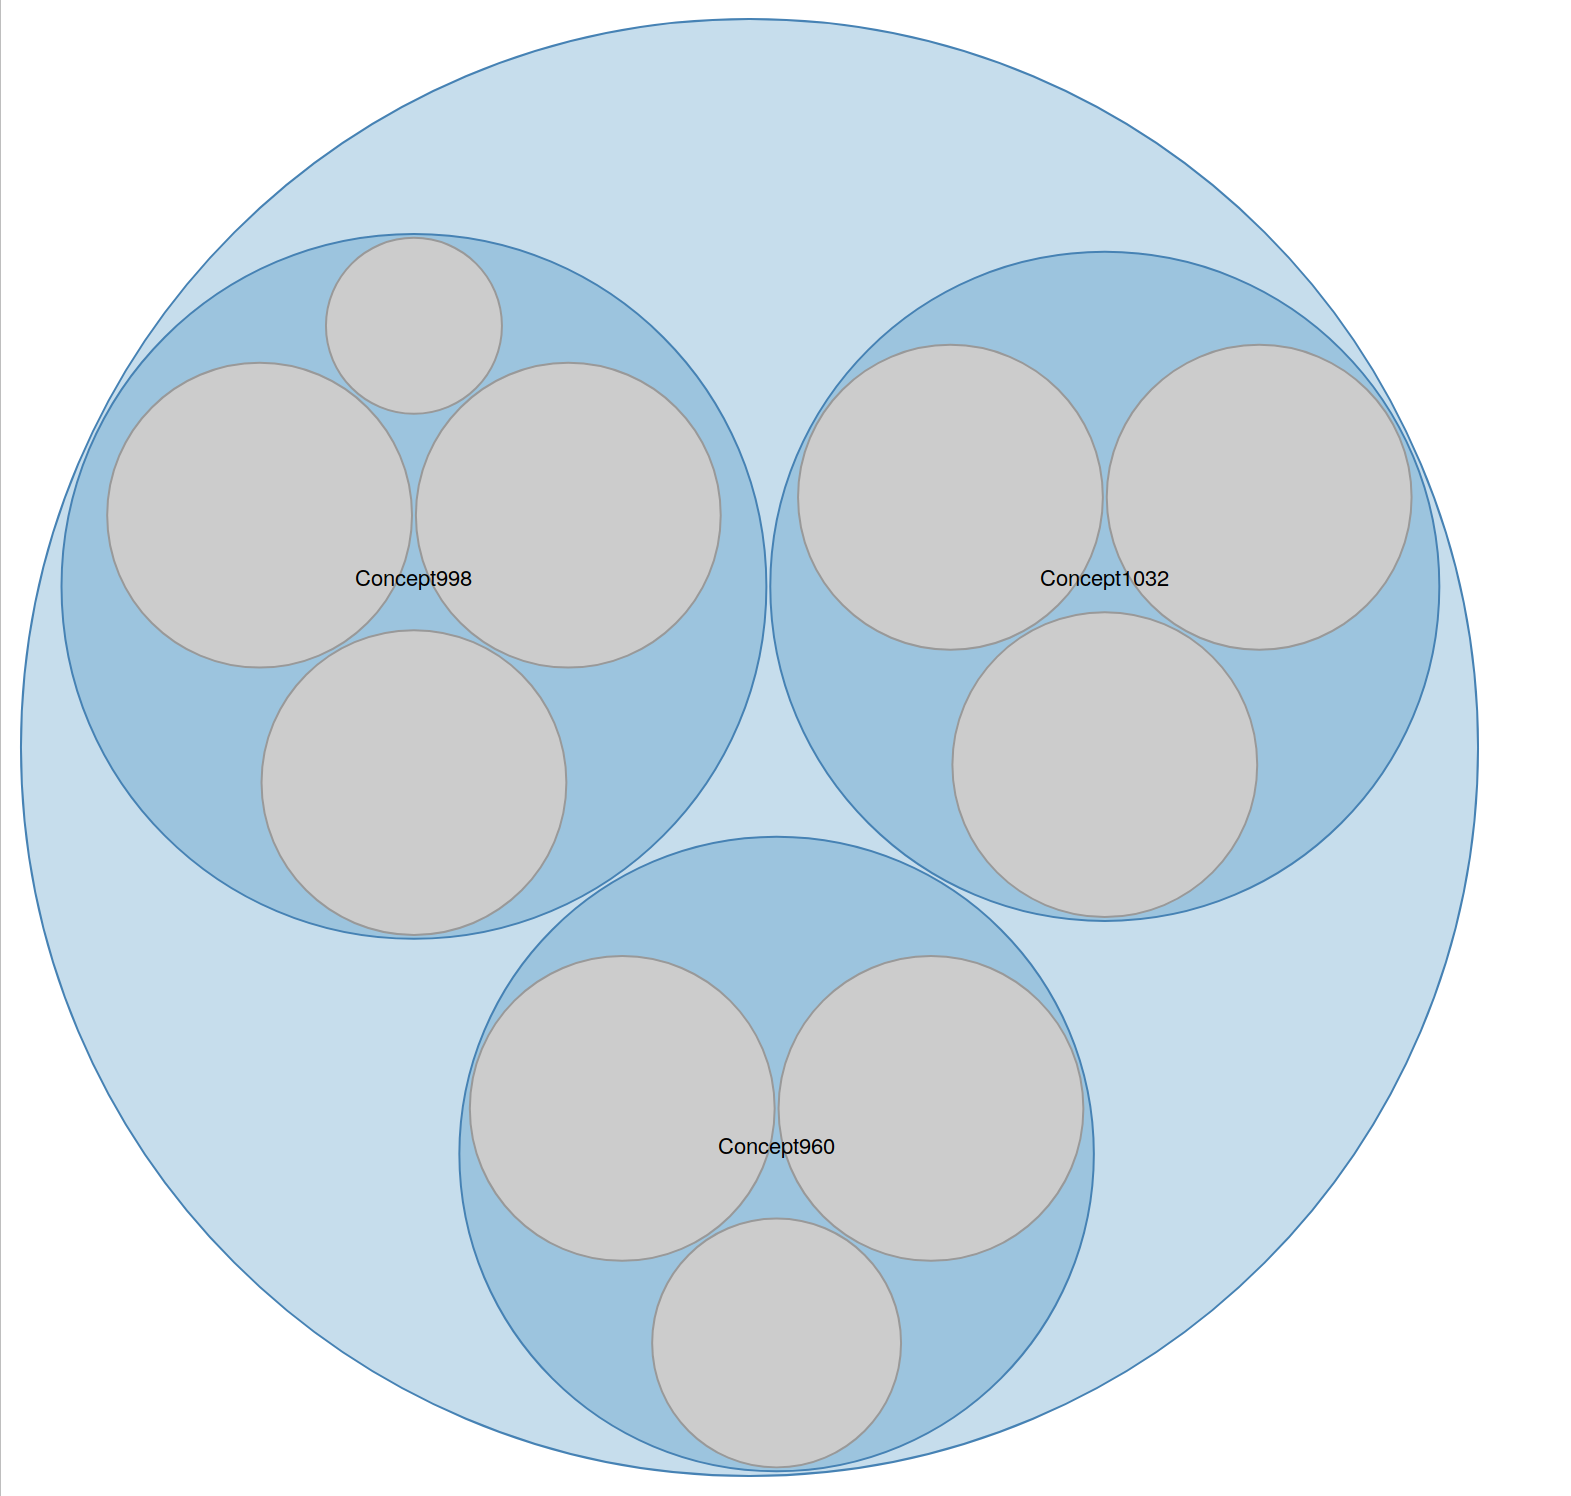
\includegraphics[keepaspectratio,width=0.48\textwidth, height=0.48\textheight]{graphics/results_trestle/trestle_10.png} \\
            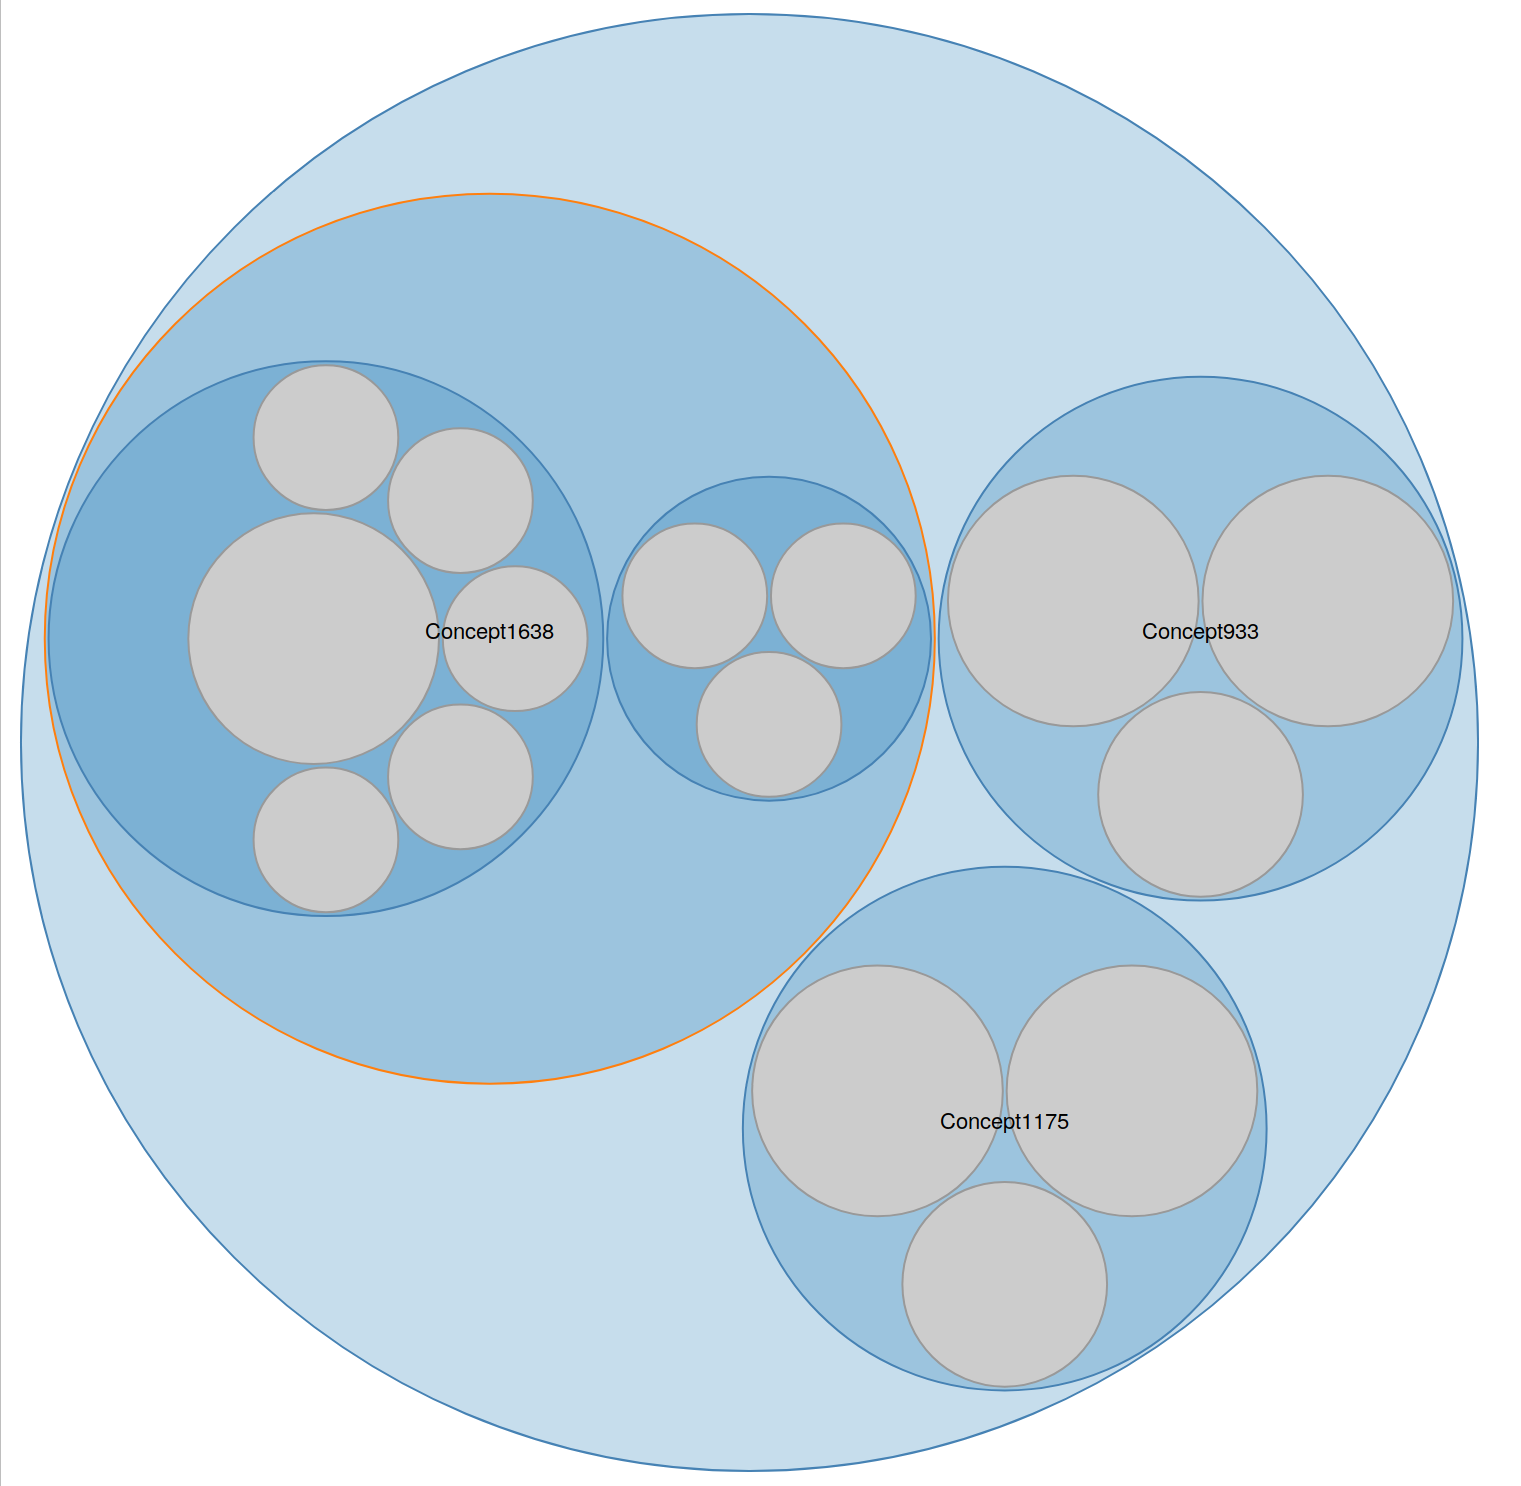
\includegraphics[keepaspectratio,width=0.48\textwidth, height=0.48\textheight]{graphics/results_trestle/trestle_33.png} \hspace{2cm}
           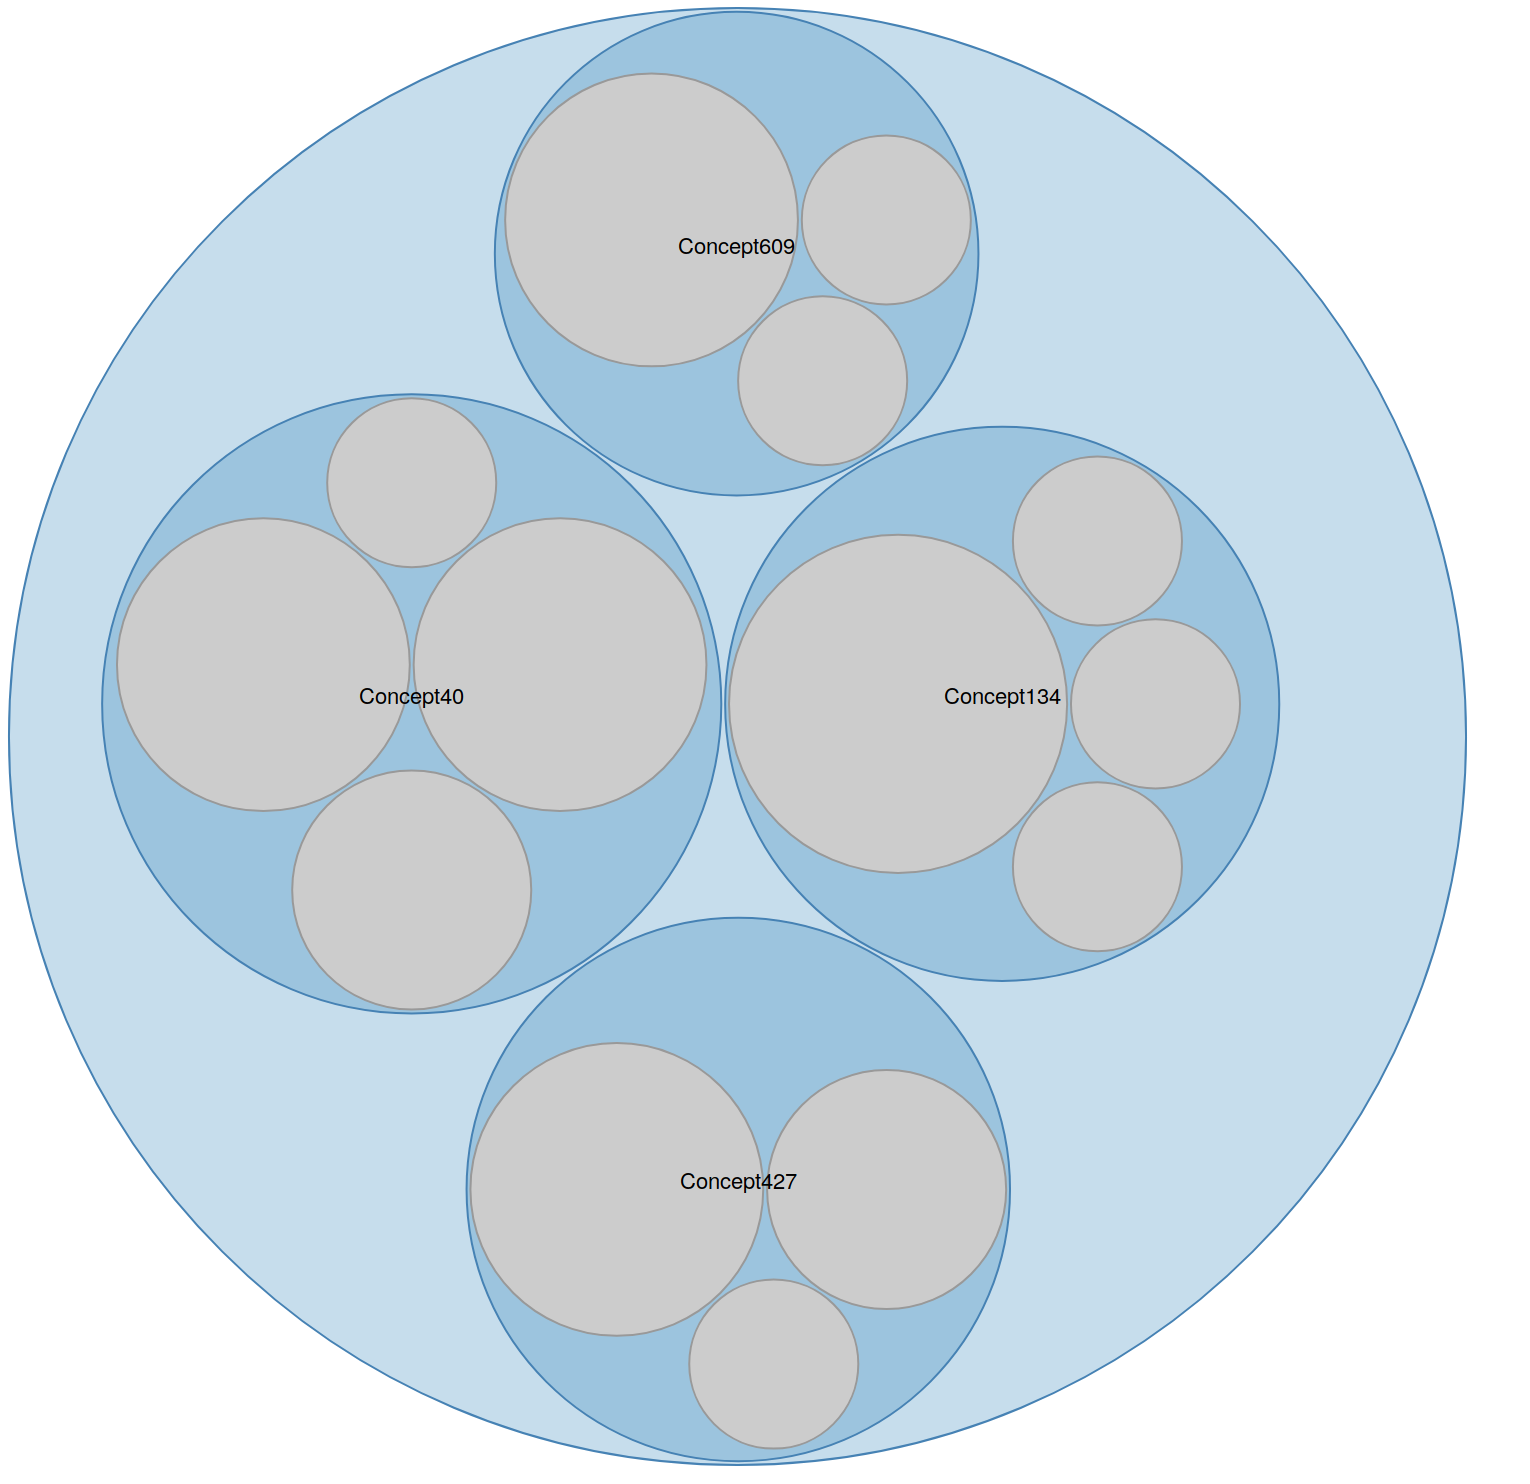
\includegraphics[keepaspectratio,width=0.48\textwidth, height=0.48\textheight]{graphics/results_trestle/trestle_50.png}
        \end{frame}{}
        
    \subsection{Issues}
        \begin{frame}{Approaches I \& II}
            \begin{itemize}
                \item[P1:] One merge per level $\Rightarrow$ not a proper tree with levels
                \item[P2:] Merges are always between two clusters
                $\Rightarrow$ Flattening
                \item[P3:] Breaks down immediately when introducing noise
                \item[P4:] First step clustering algorithms are highly dependent on hyper-parameter tuning: \\
                $\Rightarrow$ Randomized parameter search
            \end{itemize}
        \end{frame}

    \begin{frame}{Conceptual Clustering}
        \begin{itemize}
            \item Outlier detection
            \item Preprocessing e.g. list flattening
            \item weighting of attributes (reliable vs. noisy)
        \end{itemize}
    \end{frame}


\section{Conclusion}
\begin{frame}{What to achieve with thesis}
    Improve/extend the conceptual clustering framework:
        \begin{itemize}
            \item \alert{leverage graph edges/relationships to make algorithm more robust:}
                \begin{itemize}
                    \item neighbourhood
                    \item ego net
                    \item recursive feature extraction
                \end{itemize}
            \item deal with outliers
            \item cut the hierarchy tree in robust only sub-trees
        \end{itemize}
\end{frame}{}

\section{References}
    \begin{frame}
      \frametitle{References}
      \begin{tiny}
      \nocite{*}
      \printbibliography
      \end{tiny}
    \end{frame}
\end{document}